%%%%%%%%%%%%%%%%%%%%%%%%%%%%% BEGIN PACKAGE
\documentclass[11pt]{amsart}       % AMS template just for the draft
\usepackage{geometry}                 % See geometry.pdf to learn the layout options. There are lots.
\geometry{a4paper}                        % .letter or a4paper or a5paper or ... 
%\geometry{landscape}                 % Activate for for rotated page geometry
%\usepackage[parfill]{parskip}     % Activate to begin paragraphs with an empty line rather than an indent
\usepackage{graphicx}                   % FIgure
\usepackage{amssymb}                 % Math symbol
\usepackage{epstopdf}                   % for working in .pdf and  not .dvi (convert .eps, .jpg,  etc to .pdf)
\usepackage{psfrag}
\usepackage[T1]{fontenc}
\usepackage{aeguill}
\DeclareGraphicsRule{.tif}{png}{.png}{`convert #1 `dirname #1`/`basename #1 .tif`.png}
%%%%%%%%%%%%%%%%%%%%%%%%%%%%% END PACKAGE
\graphicspath{{PLOT/SinglePDGEMM/}{PLOT/VectorPDGEMM/}}

%%%%%%%%%%%%%%%%%%%%%%%%%%%%% BEGIN AUTHORS AND INSTITUTIONS
\title{Ambient: overview of the workflow and design basics}
\author[A. Kosenkov, T. Ewart, B. Bauerb, A. Kantian,  M. Troyer, T. Giarmarchi]{Alexandr Kosenkov, Timoth\'ee Ewart, Bela Bauer, Adrian Kantian, Matthias Troyer and Thierry Giamarchy }

%%%%%%%%%%%%%%%%%%%%%%%%%%%%% BEGIN AUTHORS AND INSTITUTIONS


%%%%%%%%%%%%%%%%%%%%%%%%%%%%% BEGIN MACRO
\makeatletter
\newcommand\etc{\textit{etc}\@ifnextchar.{}{.\@}}
\newcommand\eg{\textit{e.g. }}
\newcommand\ie{\textit{i.e. }}
\newcommand\cf{\textit{c.f. }}
\newcommand\df{\textit{d.f. }}
\renewcommand{\labelitemi}{$\diamond$}


\makeatother
%%%%%%%%%%%%%%%%%%%%%%%%%%%%% END MACRO
\begin{document}

%%%%%%%%%%%%%%%%%%%%%%%%%%%%% BEGIN SYMBOL
\def\cloud{\includegraphics[width=0.2cm]{FIGURES/cloud}}
%%%%%%%%%%%%%%%%%%%%%%%%%%%%% END SYMBOL
\maketitle

%%%%%%%%%%%%%%%%%%%%%%%%%%%%% BEGIN INTRODUCTION
\section{Introduction}

Over the last twenty years, the High Performance Computing (HPC) community has seen the technical evolution of hardware continuously influence the programming model.
Over this timespan, the most powerful machines have moved from shared to distributed memory architecture, with networks of
distributed memory nodes with multicore processors using optional accelerators being the current norm\cite{Top500}.  This transition took place in three distinctive steps.

First, was introduction of modular nodes based on modular blade systems in the nineties\footnote{SMP systems disappeared from theTOP 500 list 
of supercomputers in 2002}. Cutting hardware costs, this changed the programming model from shared to distributed memory API, as memory address space was
not shared among nodes and parallel processes now had to transmit data over an interconnecting network. Several technologies were designed to allow communication
between nodes (PVM, NX, Express, P4, \etc) \cite{Aoyama:1999}, in particular the Message Passing Interface (MPI) \cite{Snir:1998:MCR:552013}. which has become the
standard for coarse-grained problem ( \footnote{A number of scientific applications requiring scalability currently employ a main MPI layer, 
{ ALPS \cite{ALPS2011} for strongly correlated quantum mechanical systems ,\sc Quantum ESPRESSO} \cite{QE-2009} for quantum chemistry, Abinit \cite{ABINIT-2005, ABINIT-2009} in quantum mechanics, ScaLAPACK \cite{SCALAPACK-1997} in linear  algebra or SMILE for hypersonic rarefied flows \cite{SMILE-2005}, to give just a brief, non-exhaustive list.} The factor limiting scalability in this programming model
is the communication overhead and the workload imbalance among processes.

Secondly, the introduction of multicore technology has allowed the integration of several CPU cores into the same die, 
rendering the shared memory model of parallelization once more current. The POSIX threads library is a proven technology in this regard, offering
two possibilities: either utilize the library directly (using pThreads), or let the compiler generate a multi-threaded executable. The first option places the burden of
shared memory parallelization on the programmer, but provides good performance when well done, while the second option, called OpenMP \cite{openmp:2002},
is based on preprocessor directives and easier to use.  It is now integrated natively in all compilers, also allowing for hybrid programming, with hybrid MPI/OpenMP
being the current programming model in HPC \cite{EXASCALE-2010}.  For example, the performance of the ScaLAPACK library has been shown to improve by
employing multithreaded BLAS libraries (MKL, ESSLSMP or ACML) [A.K.: NEED CITATIONS HERE.] 
Although this ideology can yield good results, the threads management imposes an additional workload when the grain problem size becomes too fine \cite{SMITH-2001}. 

The latest step in this development is the introduction of graphics processing units (GPUs) into HPC. These devices typically perform hundreds or thousands of threads simultaneously, each applying a kernel
to a single or multiple pieces of data. (???)
As a framework to enable the use of these GPUs on a cluster, two APIs exist, CUDA \cite{CUDA2011} and OpenCL. Mixed CPU/GPU nodes can be run in hybrid mode, i.e. operations are split up
and executed asynchronously between multiple CPU cores and the GPUs. As with pThreads, the programmer can manage this by hand or delegate via preprocessor directives \cite{PGICUDAFOR2010}.
The MAGMA library \cite{MAGMA_2011} would be an example of this model.  

For the HPC developer, the challenge amidst all these advances is not just to develop code adapted to the latest hardware capabilities 
and constraints, but to address both the given bottlenecks of the algorithm, the (possibly changing)  bottlenecks of the hardware, and that these 
two may not be (or stay) congruent. Furthermore, in scientific simulations particularly, the structure of the problem has usually been
exploited to write a complex code that performs very well - on a single node. The question of how to transpose such code to a large distributed
cluster while keeping useful and well-performing design is non-trivial, as the direct approach of MPI-parallelizing each operation by hand may
be prohibitively complex and expensive.

The purpose of the paper is to present a new programming model based on a powerful oriented object (C++) framework named Ambient, that
transposes the CUDA ideology to a cluster. As in the CUDA framework, in Ambient, the developer writes kernels which are executed in parallel under
MPI groups, allocating cluster resources, dynamically if needed. The communications are assured by a nested MPI layer away from the user.
Thus, amongst its capabilities, Ambient allows a bootstrap parallelization of existing serial or shared-memory parallel code to distributed-memory systems,
where the operations that the serial code would perform at each step are collected into a stack. This operation stack is then executed, with Ambient grouping
dependent and independent operations as necessary, designating MPI processes as appropriate to each of them, and, crucially, managing data storage and
transfer between MPI processes with an eye towards keeping data volume over the network low and traffic fast. Any algorithm whose basic operations and data
objects are inhomogenous in terms of time and size requires this dynamically adaptable resource allocation in practice, which Ambient handles largely in the background.
The scientific algorithm for which Ambient was originally developed, the Density Matrix Renormalization Group (DMRG) [A.K.: INSERT CITATIONS HERE] for example has just this structure,
as its basic operations are mostly dense matrix-matrix multiplications, with the dense matrices ranging widely in size. The largest ones may necessitate distribution
over several nodes, while smaller ones may fit easily into the memory of a single node.

In the following, we will describe the general blueprint of Ambient and its' workflow, the differences to CUDA, and evaluate several basic linear algebra benchmarks.  
We will apply and illustrate our framework on basic linear algebra problems, especially on pBLAS operations.

%%%%%%%%%%%%%%%%%%%%%%%%%%%%% END INTRODUCTION


%%%%%%%%%%%%%%%%%%%%%%%%%%%%% BEGIN WORKFLOW
\section{Ambient workflow}

Before presenting various elements of Ambient in more detail, this section provides the
workflow of execution for an Ambient-parallelized application in general terms. 
As the Ambient computational architecture derives from CUDA, we start with a simplified
workflow of execution for both CUDA-enabled and Ambient enabled applications side-by-side:

\begin{table}[h]  
	\begin{center}
	 	\begin{tabular}{l l  l l} % L L  L L 
                        \hline 
                             \multicolumn{2}{c}{CUDA} &  \multicolumn{2}{c}{Ambient} \\
                             \hline
                             \multicolumn{4}{c}{  $\diamond$ Serial code}  \\
                            $\diamond$ & Kernel encountered                                  &  $\diamond$ & Kernel-pair (logistic/computa- \\
                               & & & tional) encountered \\
                               $\diamond$ &Thread block grid construction&     $\diamond$  & Kernel-pair stacked for later  \\
                                &(gridDim, blockDim)  &  &  execution  \\ 
                               $\diamond$ &  Thread blocks mapping onto de-  &  &  \\
                                & vice (GPU SMPs) &  & \\
                               $\diamond$ &  Execution of kernel: GPU SMP & & \\
                               &  executes kernel on every thread& &    \\
                               &  of corresponding thread blocks  & & \\
                               \multicolumn{4}{c}{  $\diamond$ Serial code}  \\
                               & &    $\diamond$&Stack flush signal encountered : \\
                               & & & execution of kernels \\
                                  \hline
        		 \end{tabular}  
              \caption{Workflow analogy between the execution of a CUDA and a Ambient application} \label{WORKFLOW}
	\end{center}
\end{table}

[A.K.: VERY BRIEF DESCRIPTION OF CUDA HERE] Any Ambient-parallelized operation on the other hand is broken down
in two parts:  first, a logistic kernel sets up the necessary MPI processes and prepares the data. Secondly,
a computational kernel executes the calculation, performing any necessary communication between MPI processes in the background.

In a code bootstrap-parallelized via Ambient, operations are stacked up symbolically and are actually performed when a flush signal
is encountered (accumulated execution model); contrary to CUDA, the programmer decides when to start execution.
Kernel execution is initiated along the following sequence:
(   a deeper description of the pair logistics/computational kernels is given in the next section)
\begin{itemize}
\item Execution of logistic kernel: allocation of device (MPI group) according to specified request. 
\item Execution of logistic kernel: different parts of an argument (i.e. data) passed to kernel are mapped to the different 
        work groups making up the device (i.e. the MPI group).
\item Execution of logistic kernel: selected argument's work groups are mapped onto device (MPI processes).
\item Transfer of work groups to the target processes.
\item Execution of computational kernel: MPI process executes kernel thread for work items of assigned work groups.
\end{itemize}

The main reason for the difference in workflow compared to CUDA is the scale of available resources.  As practically unlimited resources
are available for a kernel's launch, the data becomes the key factor around which Ambient's design evolves.
In particular, in order to control the data movements and resource usage, we introduce the logistic kernel and make kernel calls non-blocking. 

Generally, Ambient enabled applications operate with abstract types that already have tiled memory structure. Upon encountering a kernel operation 
call, the Ambient framework stacks the operation for later execution and proceeds in this manner through the serial code. This design
enables a high degree of reusage of the original serial code, while providing powerful instrumentation capabilities to manage resources and tune performance 
of the application overall.

The  accumulated execution model is one of the important features of Ambient, it easily accomodates another layer of parallelization, that of operations,
if that is useful for the problem at hand. Indeed several kernels can be push into the stack before the execution signal. When the framework encounters the signal to flush the stack of kernels the actual execution starts. 
The framework's engine goes through the accumulated stack  and executes all independent operations at once. Executing an operation, the engine first invokes the associated logistic kernel and allocates a specified
amount of resources for this operation. Next, the engine sets the argument's (here: the matrices) tiling using user specified work group sizes and maps resulting work groups onto allocated
processes. Now the engine can freely transfer the tiled data from previous owners to the allocated processes changing
the tile size if needed. After the transfer is complete the computational kernel kicks in behaving almost the same way as in CUDA, with work groups
simply being mapped onto threads of MPI process as if they were GPU SMP (the difference lies mainly in the user's control over the mapping of processes to work groups).

In the following sections, we elaborate on the role and functionalities of the different elements listed here.

%%%%%%%%%%%%%%%%%%%%%%%%%%%%% END WORKFLOW


%%%%%%%%%%%%%%%%%%%%%%%%%%%%% BEGIN DESCRIPTION OF THE FRAMEWORK
\section{Design of the framework}
%In this section, we describe our framework in simple terms, without  a deep technical description.
%We will focus on the main functionalities  and show the essential features.

%%%%%%%%%%%%%%%%%%%%%%%%%%%%% BEGIN CUDA IDEOLOGY SECTION
\subsection{Extending the CUDA approach} \label{CUDAIDEOLOGYSECTION}

Ambient employs an extension of the CUDA approach onto a distributed cluster. This is based on the observation that modern clusters employ many thousands of nodes, just like a GPU consists of thousands of small, simple cores, on each of which it runs an independent thread. In such a comparison however, the technical specifics of the basic cluster unit in terms of processor power, memory bandwidth, network speed, \etc  \, must be considered. 

A CPU core has much higher capabilities than a GPU core, and thus we can't simply downcast the CPU core to the GPU one.
Therefore, the scope of the data for a single CPU (on which a single Ambient thread typically runs) in Ambient is rather comparable to the capacity of CUDA's thread block or an OpenCL work group. The typical block size is $ 128 \times 128$, although, the user has full control of this size and can adapt it to the needs of the target problem. As in CUDA, work groups and corresponding grid of groups are formed in Ambient. A basic comparison between CUDA and Ambient is shown in table \ref{ANALOGY}.
Moreover the representation of the data by work group fits very well with linear algebra and the matrixes representations (basic types).

\begin{figure}[t]
	\begin{center}
	                  %psfrag for changing the layout
	                  \psfrag{New data layout}{\tiny{new layout}}
			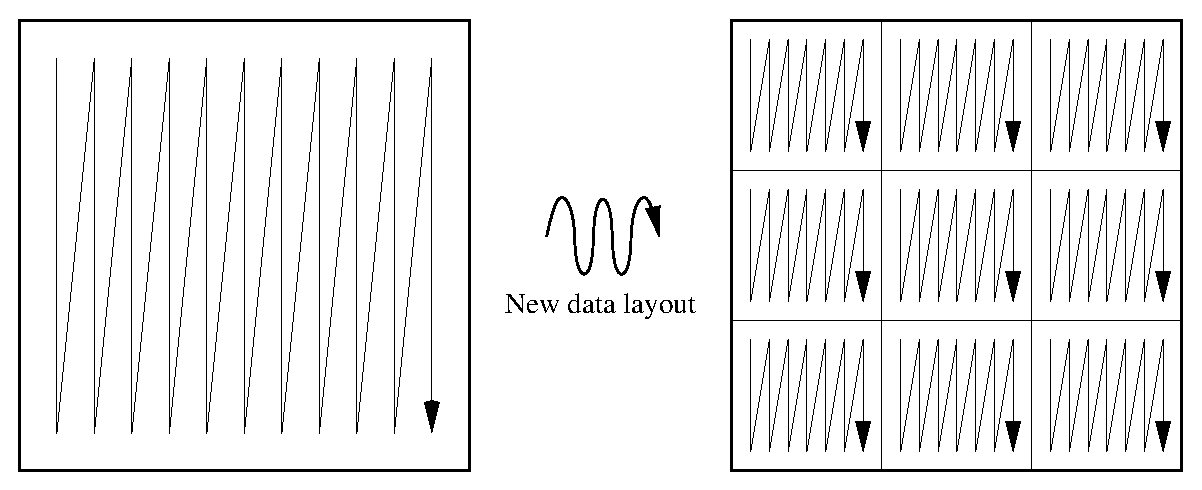
\includegraphics[scale=0.44]{FIGURES/MemMatrix.eps} 
	\end{center}
          \caption{Representation of the data layout inside the memory. Instead of the single contiguos block's layout we use tiled layout.}
          \label{MEMMATRIX}
\end{figure}

The work group approach imposes the data layout of the framework. The standard math libraries impose both column-major-order as well as a contiguous memory order on a matrix storage (figure \ref{MEMMATRIX}).

Therefore, we keep the column order but do not conserve a full contiguous buffer. As in the PLASMA library \cite{LTAIEF-2011}, we choose
a tile data layout. It allows to avoid penalties due to NUMA nature of memory allocation on the CPU (section \ref{MPIABSTRACTION}) and, naturally, this data layout supports the work group representation of execution, as shown in Fig. \ref{CUDAANALOGY}. 

In CUDA and OpenCL, the execution model imposes kernel initialization with the appropriate resources (\eg block and grid dimensions),
after which the user does not have to explicitly manage the memory transfer inside the GPU; due to the distributed memory of clusters and the frequently heterogeneous nature of processing units we need both fine-grained control of the work group per process assignement as well as of the memory transfer operations. That should be done in a simple, automatic yet flexible way. In order to achieve this goal we split the kernel invocation into two parts.

First, we prepare the memory of corresponding work groups. Then we execute our numerical operations \eg a matrix multiplication in the following sequence \footnote{From here onwards, we will illustrate the execution model through parallel matrix addition or multiplication.}:
\begin{enumerate}
	\item A logistic kernel; where we select the number of processes, and map the data onto them.
	\item A computational kernel; where we execute required computational operations (similar to the CUDA-kernel).
\end{enumerate}

Thus, every operation (\eg multiplication, addition, or more sophisticated linear algebra operations) will have an associated logistic and computational kernel. 

\newpage

\begin{figure}[!t]
	\begin{center}
           	        \psfrag{Ambient representation}{\tiny{\hspace{-0.4cm}Ambient representation}}
           	        \psfrag{CUDA/OpenCL representation}{\tiny{\hspace{-0.9cm}CUDA/OpenCL representation}}
	                 \psfrag{Associated mapping of the data with Ambient}{\tiny{\hspace{+0.15cm}Associated data mapping}}
	                 \psfrag{1x1 workgroup}{\tiny{\hspace{-0.5cm} \vspace{-0.1cm}1x1 workgroup}}
	                  \psfrag{of Ambient}{\tiny{\hspace{-0.4cm}\vspace{-0.9cm} of Ambient}}
	                  \psfrag{Workgroup of 4X4 threads}{\tiny{\hspace{-0.5cm} \vspace{-0.1cm}4x4 workgroup}}
	                  \psfrag{of CUDA}{\tiny{\hspace{-0.25cm}of CUDA}}
	                  \psfrag{Scope of GPU thread (left)}{\tiny{\hspace{-0.25cm}GPU scope left}}
	                  \psfrag{CPU (right)}{\tiny{\hspace{-0.7cm}CPU scope right}}       
		        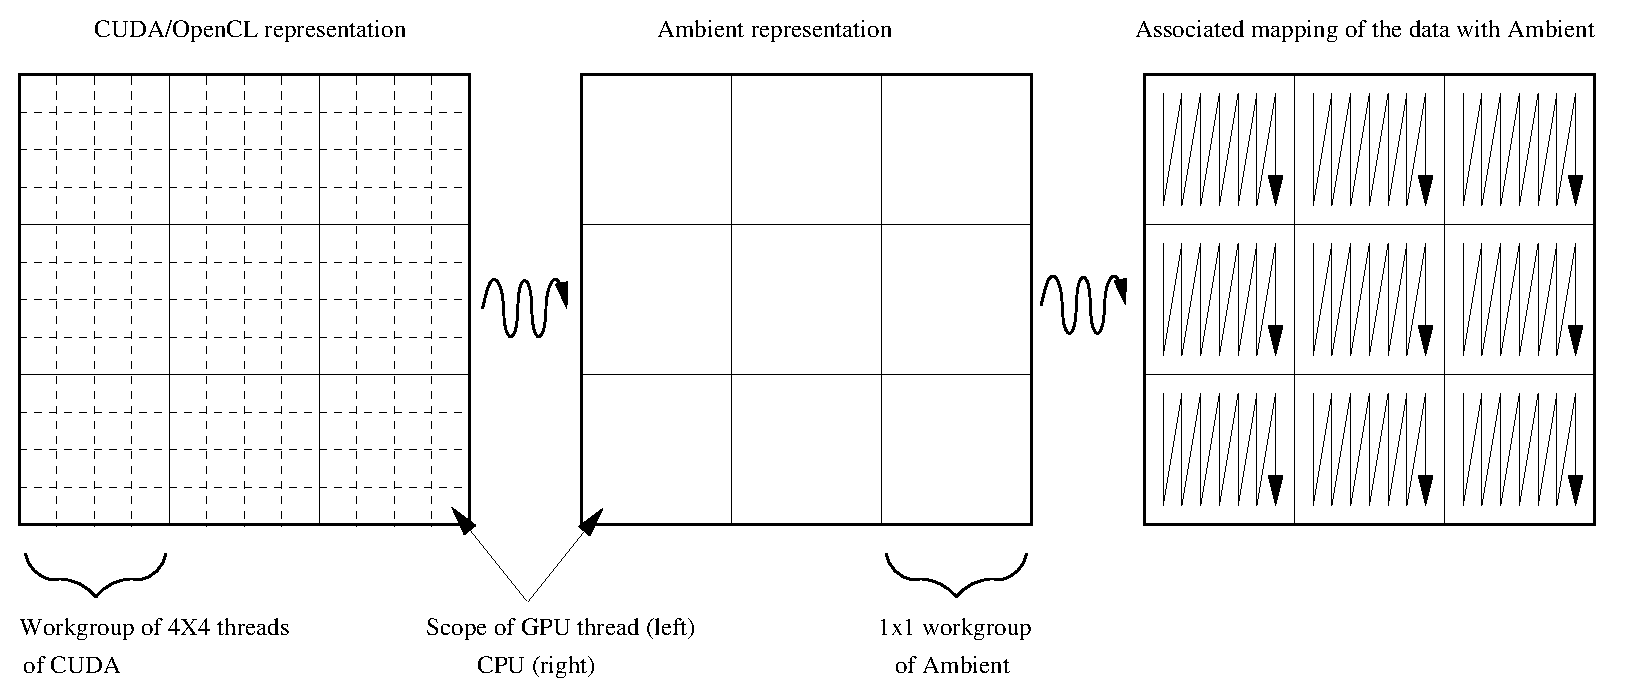
\includegraphics[scale=0.44]{FIGURES/CUDAanalogy.eps} 
	\end{center}
          \caption{Similarity between CUDA's thread grid and Ambient's work group grid (with tiles mapped to work groups).}
          \label{CUDAANALOGY}
\end{figure}
\begin{table}[h]
	\begin{center}
	 	\begin{tabular}{c  c  c}
		 	                                                      & CUDA/OpenCL                                & Ambient            \\  \hline 
			 Device                                        & GPU or CPU (socket)   & Cluster               \\  
			  Entity  of Calculation               & GPU-Thread                                      & CPU-Thread     \\  
			 \begin{tabular}{c}
			 Scope of the \\ 
			 entity calculation  
                             \end{tabular}
                             &  Buffer entry                            & Full buffer \\
			 Execution model                       & Kernel                                                &  \begin{tabular}{c}  Logistic and \\ computational kernel   \end{tabular} \\
			 work group-ID                           &  \texttt{blockIdx}                                 & \texttt{get\_block\_id(A)}   \\  
			 work group size                        &  \texttt{blockDim}                               & \texttt{get\_mem\_dim(A)}      \\  
			 grid size                                     &  \texttt{gridDim}                                  & \texttt{get\_grid\_dim(A)}  \\ \hline

		\end{tabular}
		\caption{Analogy between the Ambient framework and  the CUDA and OpenCL ideology.  \texttt{A} is the associated matrix to the  logistic and computational kernel.  
		The access of the cartesian values are done by the classical operator C/C++ \guillemotleft.\guillemotright     \, \eg \texttt{get\_mem\_dim(A).x}  	\label{ANALOGY}}
	\end{center}
\end{table}

\newpage

\subsubsection{The logistic kernel} The role of the logistic kernel is to initialize memory and work groups for execution. It consists of creating an MPI-group and mapping the data to the group with the appropriate pattern (for example 1D/2D block-cyclic distribution or the row/column-wise block distribution).  The selection of the group is done by issuing an SQL-like request. Afterward the data is mapped onto this newly created group using surjective assignments. Both these functionalities are described in section \ref{SQLSECTION}.

In linear algebra, the optimal distribution in terms of load balancing often is the 2D block-cyclic distributions, but in general it depends on the target algorithm. For example, for the QR factorization \cite{DEMMEL-2008} it can be demonstrated that the row-wise distribution is superior to the 2D block-cyclic decomposition for matrices with more rows than columns. Switching from one distribution scheme to another is a challenge for ScaLAPACK while can be easily accomplished with Ambient.
 \begin{table}[h]
	\begin{center}
	 	\begin{tabular}{l l }
                           \hline 
                           \textbf{Logistic kernel }  Algorithm of the addition logistic kernel  &    \\ \hline
                           \textbf{Require}                 A class \texttt{Matrix} that adheres the Ambient architecture  &  \\
                           \begin{tabular}{c l} 
                           \tiny{1:} &  Addition\_logistic(Matrix $A$,  const Matrix $B$)  \\
                           \tiny{2:} &  SQL request for $N$ processors selection   \\
                           \tiny{3:} &  Perform 2/1-D cyclic distribution of the Matrix $A$  $\vartriangleright$ Note: the distribution \\
                                         & is performed with the number of processors selected inside the SQL request. \\
                           \tiny{4:} &  Perform 2/1-D cyclic distribution of the Matrix $B$ \\
%                           \tiny{5:} &  Perform 2/1-D cyclic distribution of the Matrix $C$ \\ 
                           \end{tabular} & \\ \hline
		 \end{tabular}  
		 \caption{Logistic kernel associated to the matrix multiplication or  the addition.  \label{LKERNEL}}
	\end{center}
\end{table}

\subsubsection{The computational kernel}  After the logistic kernel has been executed, we are ready for the computational kernel. The mode of execution is similar to the CUDA API with a few specificities. In the CUDA parallel computing model, the programmer writes a single thread program, using the CUDA-API,  after which the GPU runs multiple instances of this thread in parallel. We transpose this approach into Ambient. Nevertheless, we should not forget the data scope of a single CPU "thread" in Ambient roughly corresponds to the scope of a full OpenCL work group. 

We have introduced a keyword (like the \texttt{const} keyword) named \texttt{pinned}. This keyword indicates to the framework that the kernel must be executed over all work groups of the marked argument. Inside the kernel we use Ambient API, analogous to CUDA, in order to obtain necessary information about the work groups (position, dimension and so on). Those are partly lister in the table \ref{ANALOGY}.  For illustration purposes, the computational kernel (table \ref{CKERNEL}) of an addition of the two matrices associated with previous example of the logistic kernel is presented in the table \ref{LKERNEL}.
\begin{itemize}
\item Line 1: the signature of the computational kernel must be the same as of the associated logistic kernel. Here we will also include the use of the \texttt{pinned} keyword indicating that the execution should be performed over the marked argument's work groups.
\item Line 2: the cartesian coordinates of the work group are obtained from the Ambient instruction \texttt{get\_block\_id(A).x}  for $i$ and \texttt{get\_block\_id(A).y}  for $j$. \label{CURRENT}
\item Line 3 to 5 : we refer to the work group $i,j$ via the temporary variable $A_{ref}$ using the Ambient instruction \texttt{current(A)(i,j)}. Note that if the process requires data outside of its scope the remote access will be performed in the background (see section \ref{MPIABSTRACTION} for details).
\item Line 6 to 8 : the addition is performed by looping over all elements inside the work group.
\end{itemize}

 \begin{table}[t] 
	\begin{center}
	 	\begin{tabular}{l l }
                           \hline 
                           \textbf{Computatiomal kernel }  Algorithm of the addition computational kernel  &    \\ \hline
                           \textbf{Require}                 A class Matrix  that adheres the Ambient architecture  &  \\
                           \begin{tabular}{c l} 
                               \tiny{1:} &  Addition\_computational(Matrix $A$,  \texttt{pinned const}  Matrix $B$) \\
                               \tiny{2:} &  Get the cartesian coordinate $i,j$ of the work group \\ 
                               \tiny{3:} &  Refer  the  work group$(i,j)$  of A into $A_{ref}$ \\
                               \tiny{4:} &  Refer  the  work group$(i,j)$  of B into $B_{ref}$ \\
%                               \tiny{5:} &  Refer  the  work group$(i,j)$  of C into $C_{ref}$  \\
                               \tiny{5:} &  \textbf{for} $k$ from $0$ to total size of the work group \textbf{do} \\
                               \tiny{6:} & \hspace{0.2 cm}   $A_{ref}[k] \, + \!\! = B_{ref}[k]$ \\
                               \tiny{7:} &  \textbf{end for} \\                               
                          \end{tabular} & \\ \hline
		 \end{tabular} 
		 \caption{Algorithm of the computational kernel associated to matrix addition.   \label{CKERNEL}}
	\end{center}
\end{table} 

As it was shown for the matrix addition, we can recode other linear algebra solvers using Ambient's API. For the presentation of our framework, we will focus on the MPI version of BLAS named pBLAS \cite{SCALAPACK-1992}, as well as Strassen-like recursive reduced-multiplication algorithms.

%\begin{table}[h]
%	\begin{center}
%	 	\begin{tabular}{c  c  c}		 	                                                             & CUDA/OpenCL                                 & Ambient                               \\  \hline 
%			 work group-ID                                  &  \texttt{blockIdx}                                 & \texttt{get\_block\_id(A)}   \\  
%			 work group size                               &  \texttt{blockDim}                               & \texttt{get\_mem\_dim(A)}      \\  
%			 grid size                                            &  \texttt{gridDim}                                  & \texttt{get\_grid\_dim(A)}  \\ \hline
%				\end{tabular}
%		\caption{Analog�y between Ambient and  the CUDA/OpenCL ideology. \texttt{A} is the associated matrix to the present logistic and computational kernel.  The access of the cartesian values are done by the classical operator C/C++ \guillemotleft.\guillemotright     \, \eg \texttt{get\_mem\_dim(A).x}  } 	
%		\label{ANALOGY2}
%	\end{center}
%\end{table}


%%%%%%%%%%%%%%%%%%%%%%%%%%%%% END CUDA IDEOLOGY SECTION

%%%%%%%%%%%%%%%%%%%%%%%%%%%%% BEGIN SQL SECTION

\subsection{SQL resource management}  \label{SQLSECTION}
 In the previous section, we have introduced the logistic kernel and its role in resource initialization for the execution of the computational kernels. 
 One of Ambient's main qualities is the ability to perform dynamic management of the CPU resources on a cluster. To facilitate this, we have integrated an SQL parser from \cite{SQLite} into Ambient. Using this parser we select the desired number of processors according the SQL string supplied to the logistic kernel. 

At the beginning of the application's execution, the global MPI group is created, nameed \texttt{ambient}. In order to create nested groups we have used the ability of MPI to construct a new MPI group on top of the parent group (chapter 6 of \cite{MPI-2002}). We encapsulated this into the framework controlling it via the mentioned SQL request mechanism. It enables simple yet flexible control over the resources.  
An example request for the addition kernel would be

\begin{eqnarray}
       & &\texttt{scope\_select("\textit{N} from ambient as addition\_group }   \label{SQL1} \\
       & &\texttt{	where master is 0")}, \nonumber
\end{eqnarray}
This query, via \texttt{scope\_select}, will select \texttt{\textit{N}} processors from the global \texttt{ambient} MPI group. The newly created group then is 
accessible under the name \texttt{addition\_group}, its master process will have local rank 0 (see Fig. \ref{MPIGROUP}).

\begin{figure}[b]
	\begin{center}
           	         \psfrag{Data distributed over work group}{\tiny{\hspace{-0.5cm}Data distributed over work group}}
	                  \psfrag{Local MPI rank}{\tiny{Local MPI rank}}                
	                  \psfrag{Ambient master proc}{\hspace{-0.8cm} \tiny{Ambient master proc}}        	                  
	                   \psfrag{Ambient MPI group, N process}{ \tiny Ambient MPI group, cardinal $N$ process}
	                   \psfrag{Local rank}{\tiny Local rank}
	         	         \psfrag{0}{\tiny{0}}
	                  \psfrag{1}{\hspace{-0.05cm}\tiny{1}}
	                  \psfrag{2}{\hspace{-0.15cm} \tiny{2}}
	                  \psfrag{MPI group creation}{ \hspace{-0.5cm} \tiny  Group creation}
	                  \psfrag{from the SQL request}{ \hspace{-0.6cm} \tiny  from SQL request}
	                  \psfrag{Mapping of the work group throw}{ \hspace{-0.6cm} \tiny  Mapping of the work group throw}
	                  \psfrag{the mpi GROUP created}{\tiny the new MPI group}
	                 \psfrag{(0,0)}{\hspace{-0.25cm} \tiny (0,0)}
	                 \psfrag{(0,1)}{\hspace{-0.25cm} \tiny (0,1)}
		        \psfrag{(0,2)}{\hspace{-0.25cm} \tiny (0,2)}
		        \psfrag{(1,0)}{\hspace{-0.25cm} \tiny (1,0)}
		        \psfrag{(1,1)}{\hspace{-0.25cm} \tiny (1,1)}
		        \psfrag{(1,2)}{\hspace{-0.25cm} \tiny (1,2)}
	                 \psfrag{(2,0)}{\hspace{-0.25cm} \tiny (2,0)}
		        \psfrag{(2,1)}{\hspace{-0.25cm} \tiny (2,1)}
		         \psfrag{(2,2)}{\hspace{-0.25cm} \tiny(2,2)}
                           \psfrag{n}{\hspace{-0.25cm} \tiny $n$}
	                  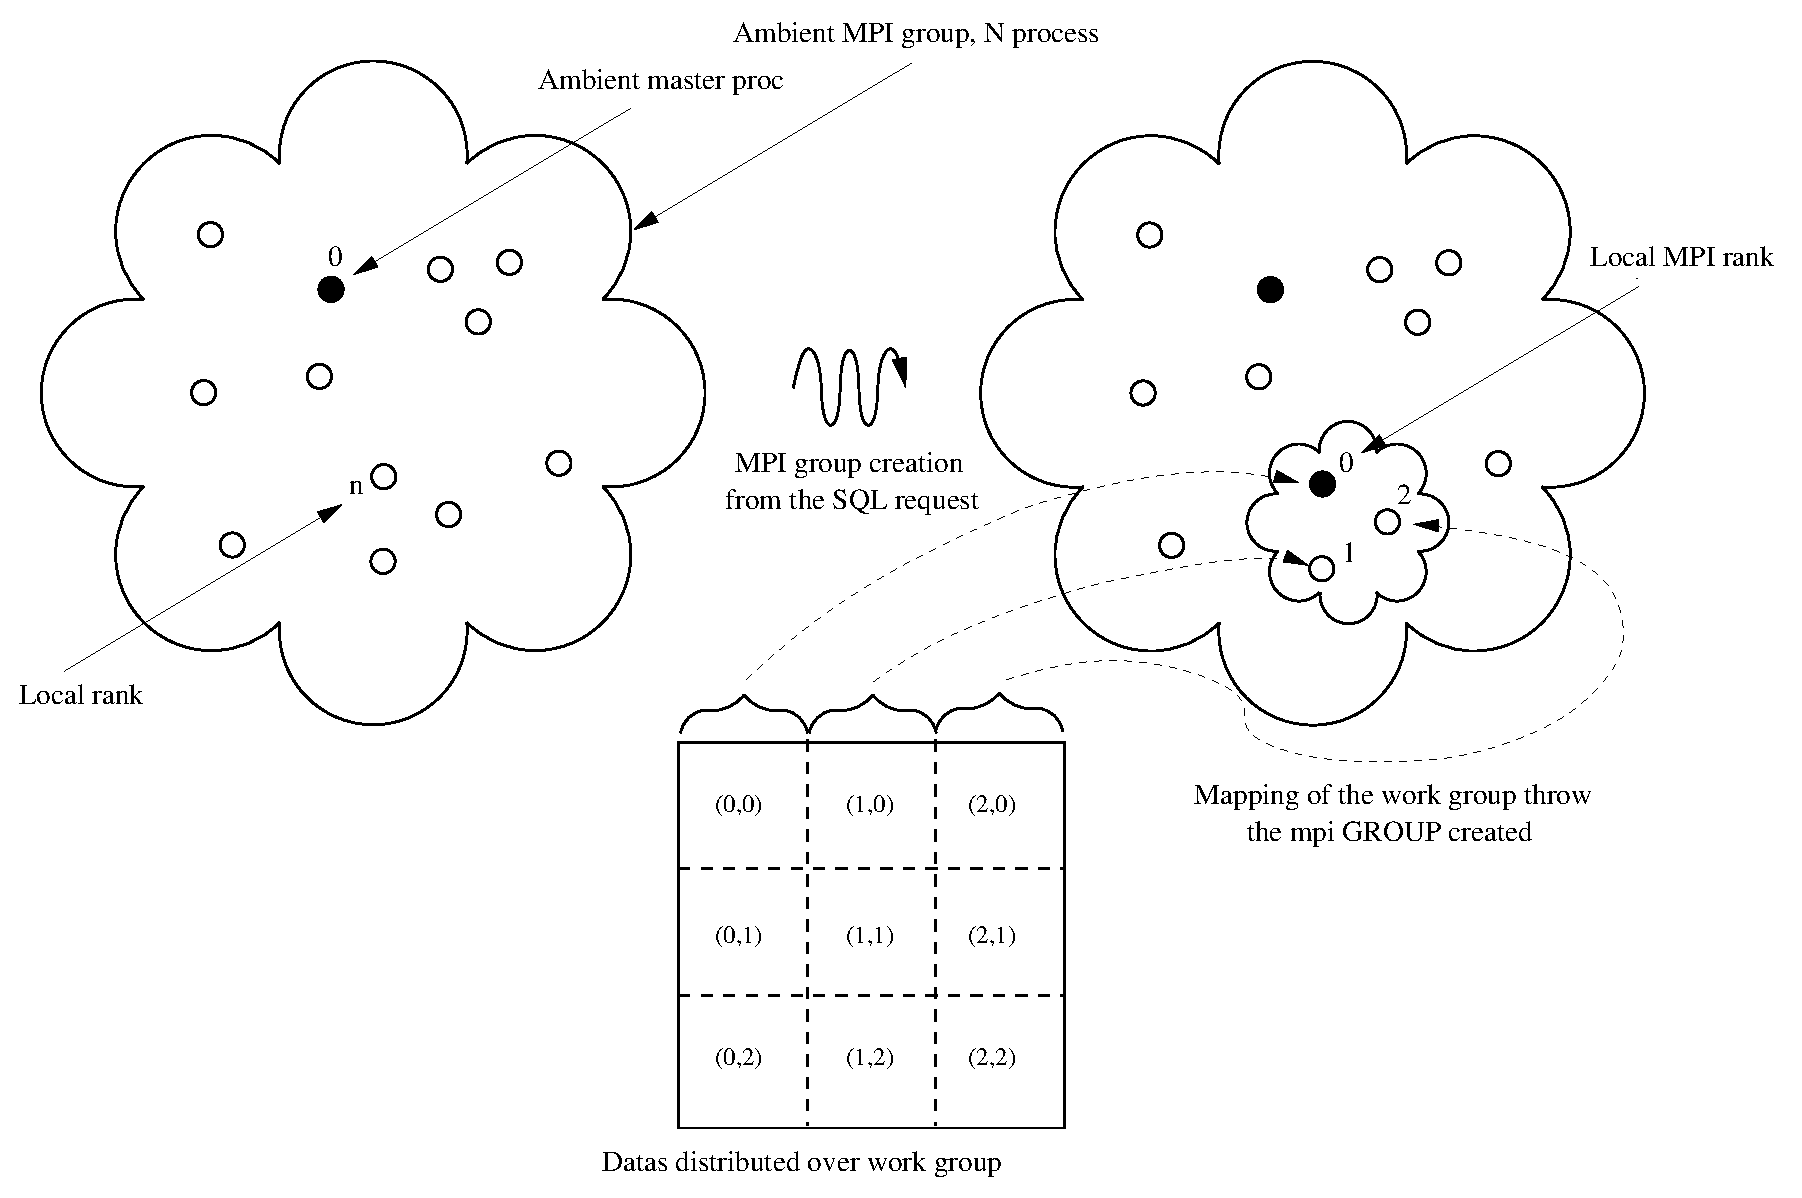
\includegraphics[scale=0.35]{FIGURES/MpiGroupData.eps} 
	\end{center}
          \caption[]{Creation of an MPI group using SQL request, with \hbox{\cloud \hspace{0.02cm}} representing an MPI group with its own communicator;  $\bullet$ represents the master 
          process inside the group whereas the $\circ$ are the associated slave processes inside the corresponding group. In this example the matrix is mapped block by block onto the processors using 1D column-cyclic distribution.}
          \label{MPIGROUP}
\end{figure}

After the SQL request section, the data is being mapped to the processes of the newly created MPI group in terms of work groups. Frequently the algorithm would be simply 1D or 2D block-cyclic distribution, the algorithm of which is described in table \ref{2DCYCLIC} (\cf Fig. \ref{MPIGROUP}). After the actual transfer, those processes will become the primary owners of their data in terms of storage and handling. With Ambient, every operation is associated with a pair of logistic and computational kernels - that is, there will be multiple SQL requests. In order to create new groups, processes from the parent group are being selected in queue fashion until all processes of the group have been selected. If more groups are required, the selection restarts from the beginning of the queue, thereby making those processes selected again simultaneous members of several groups. 

Every new group will have its own intra-communicator (allowing intra-group communication) as well as an inter-communicator (allowing communication between groups).

 \begin{table}[t] 
	\begin{center}
	 	\begin{tabular}{l l }
                           \hline 
                           \textbf{Assign workgroup}  Algorithm of the 1/2-D assign function  &    \\ \hline
                           \textbf{Require}        An new MPI group obtained by an SQL request  &  \\
                           \begin{tabular}{c l} 
                               \tiny{1:} &  Initialize $i$ in function of the new MPI rank  of the new group \\
                               \tiny{2:} &  Initialize $j$ in function of the new MPI rank  of the new group  $\vartriangleright$ Note:   \\
                                             &  the initialization of $i,j$ will fix   the distribution (1D or 2D) \\
                               \tiny{3:} &  \textbf{for} from $i$  to the number of the work group on $x$ \textbf{do} \\
                               \tiny{4:} &  \hspace{0.2 cm}  \textbf{for} from $j$  to the number of the work group on $y$ \textbf{do} \\
                               \tiny{5:} & \hspace{0.4 cm}    Assign the work group $(i,j)$ to the corresponding process\\
                               \tiny{6:} &   \hspace{0.2 cm}    \textbf{end for} \\
                               \tiny{7:} &  \textbf{end for} \\                               
                          \end{tabular} & \\ \hline
		 \end{tabular} 
		 \caption{Algorithm of the distribution of the work group into the new MPI group.   \label{2DCYCLIC}}
	\end{center}
\end{table} 

During execution, many groups will be created in practice, and data will have to be moved between groups.
To obtain better performance and to reduce the number of data transfers between groups, there are additional possible settings for the SQL request. For example, consider the previous illustration for the SQL request in case of the matrix addition operation ($ A \, +\!\!\!= B$).
If matrix $A$ has already been created and mapped on specific processors, the logistic kernel can create an MPI group as a subset or superset of the previous owner group (created in the previous operation), thereby avoiding superfluous data transfer. The concrete SQL request would be as follows:
 
\begin{eqnarray}  \label{SQL2}
         & & \texttt{scope\_select("\textit{N} from ambient as addition\_group }\\ 
         & & \texttt{	where master is 0 where breakdown contains" + get\_id(\textit{A})}), \nonumber
\end{eqnarray} 
The function \texttt{get\_id(\textit{A})} will get a tag  of \texttt{\textit{A}} to obtain its current binding.
 
%\begin{figure}[h]
%	\begin{center}
%			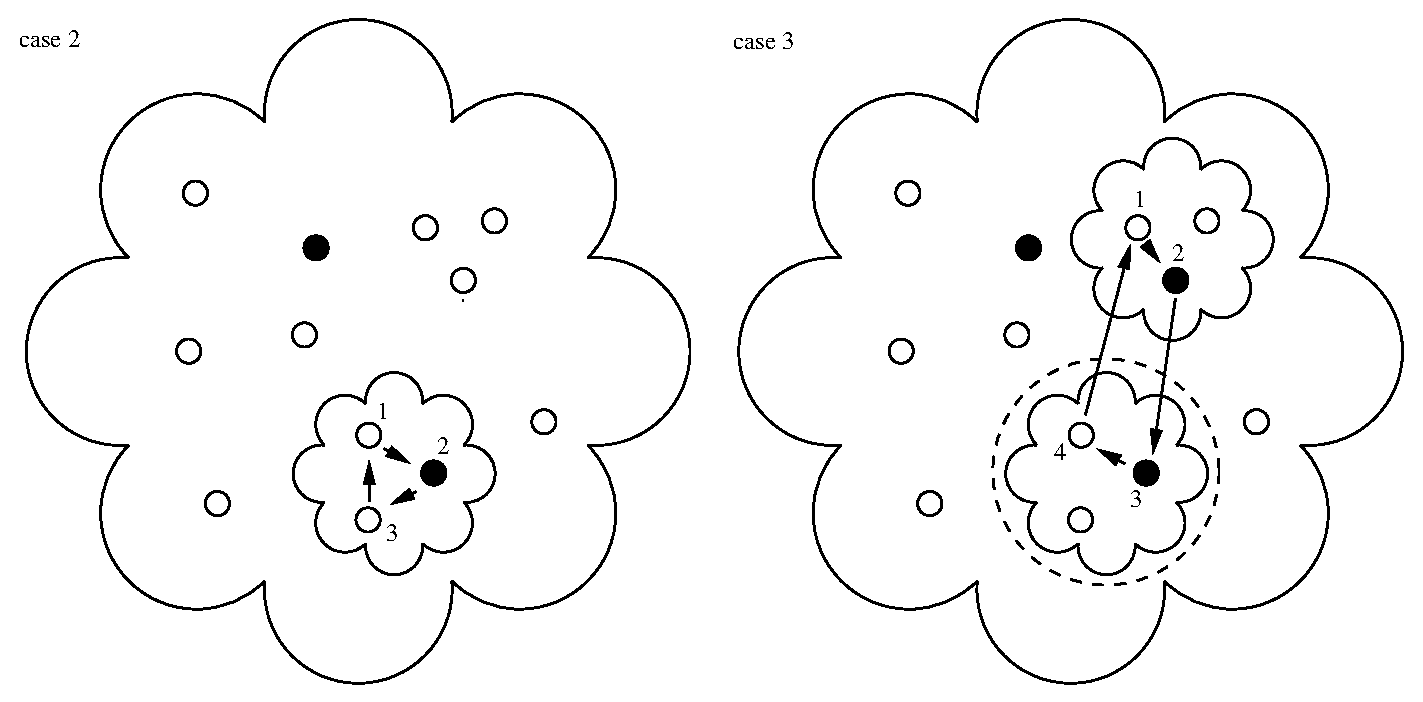
\includegraphics[scale=0.35]{FIGURES/ComGroup.eps} 
%	\end{center}
%          \caption{Data exchange inside the group.}
%          \label{COMGROUP}
%\end{figure}

%%%%%%%%%%%%%%%%%%%%%%%%%%%%% END SQL SECTION

%%%%%%%%%%%%%%%%%%%%%%%%%%%%% BEGINNING EXECUTION AND OPERATIONS SCHEDULING SECTION
\subsection{Execution model and Operations scheduling}
In a typical HPC application, the programming model imposes parallel execution of every function of the code, with data granularity imposing the details 
of the parallelization. In Ambient, we have made a scheduler that privileges a queue execution model where operations
are stacked up in a list first and are executed afterwards according to the respective logistic/computational kernel.

Any HPC application can be decomposed into a set of functions performing numerical operations. Let's start from a basic example, where we want to perform the three following operations :

\begin{eqnarray} 
\text{Operation 1:} & & A + \!\! =  B, \label{3OPERATIONS}  \\
\text{Operation 2:} & & A \times \!\!= \lambda,   \nonumber  \\ 
\text{Operation 3:} & & C \times \!\!= D. \nonumber
\end{eqnarray}
with $A$, $B$, $C$ and $D$ being some matrices and $\lambda$ being some scalar.

Conventionally, each of these three operations would be executed in parallel, one after another. Transposing into Ambient's conception means associating each operation with a logistic and a computational kernel. Considering the example (\ref{3OPERATIONS}), one would invoke the following \texttt{push} function:

\begin{eqnarray}
     \texttt{push(Addition\_logistic, Addition\_computional, \textit{A}, \textit{B})},
\end{eqnarray} 

with the appropriate logistic and computational kernels \texttt{Addition\_logistic} and \texttt{Addition\_computational}  (c.f. table \ref{LKERNEL} and \ref{CKERNEL}), followed by the arguments \texttt{\textit{A}} and \texttt{\textit{B}}. This way, operations, such as those in (\ref{3OPERATIONS}), will stack up during execution of the application. At any time then, the operations on the stack would be available for execution through the basic Ambient instruction

\begin{eqnarray}
      \texttt{playout()},
\end{eqnarray} 

although ideally this command would be invoked at the end, when all operations have been pushed onto the stack.
The \texttt{playout()} command triggers the Ambient engine to scan through the operation stack, identify the independent operations and mark dependencies. Next, a dedicated MPI packet manager\footnote{a tool managing the communication between processors.} (see section \ref{MPIABSTRACTION})  is added for each operation, and all logistic kernels for independent operations are executed. Next the computational kernels of these independent operations are executed. Following the completion of those, Ambient iterates over the remaining operations and takes the chunk of newly independent operations (whose dependencies were satisfied) and repeats the cycle, transporting the necessary data to the new groups after the execution of logistic kernels is complete. In the case of data dependency, the data transfer is handled by the packet manager. When all computational kernels have been executed, the stack is cleaned. The schematic overview of stack execution is presented in Fig. \ref{EXECUTION} .

Overall, Ambient employs a "single kernel multiple data" parallelism model that is used simultaneously over many process groups with different kernels and data sets.

\begin{figure}[h]
	\begin{center}
	      	        \psfrag{Operation 1}{\tiny{Operation 1}}
		        \psfrag{Operation 2}{\tiny{Operation 2}}
		        \psfrag{Operation 3}{\tiny{Operation 3}}
		        \psfrag{l/c kernel 1}{\tiny{l/c kernel 1}}
                           \psfrag{l/c kernel 2}{\tiny{l/c kernel 2}}
                           \psfrag{l/c kernel 3}{\tiny{l/c kernel 3}}
                           \psfrag{Ambient}{\tiny{Ambient}}
                           \psfrag{Schedule}{\tiny{Schedule}}
                           \psfrag{Dependency}{\tiny{Dependency}}
                           \psfrag{Time}{\tiny{Time}}
                           \psfrag{Evolution}{\tiny{evolution}}
                           \psfrag{Mapping and execution}{\tiny{Mapping and execution}}                          
                           \psfrag{Ambient execution}{\tiny{Ambient execution}}                          
                           \psfrag{Usual execution}{\tiny{Usual execution}}                          
	                  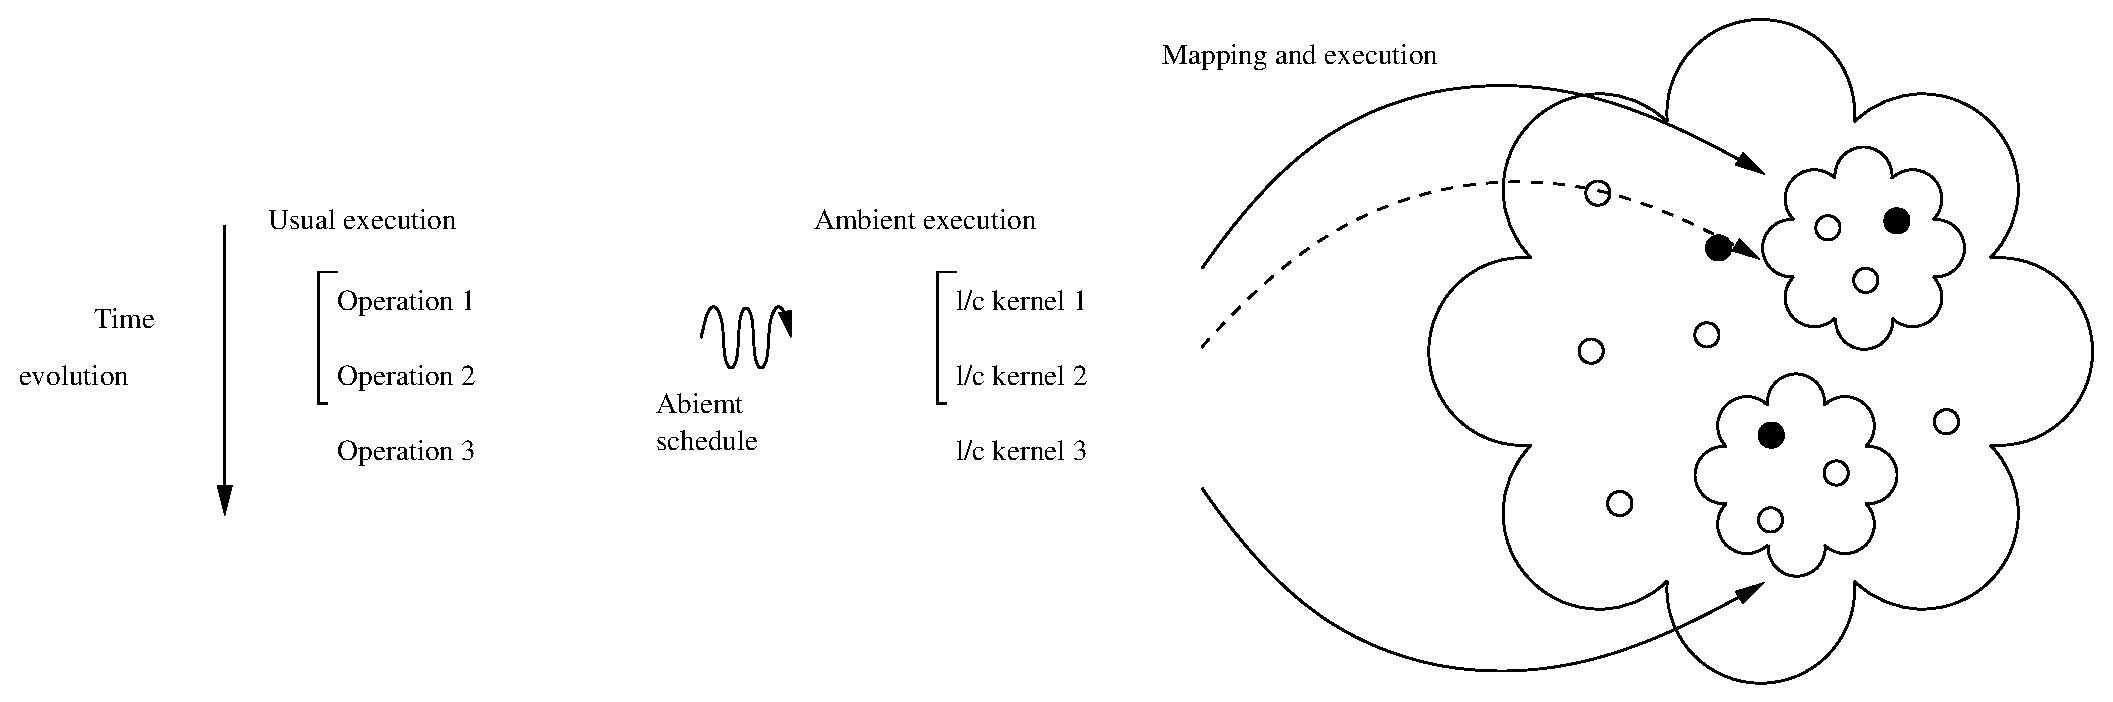
\includegraphics[scale=0.35]{FIGURES/execution.eps} 
	\end{center}
          \caption{Ambient scheduler's workflow model. In the classical approach (left) the operations will be executed in parallel step by step disregarding the dependencies (marked by the symbol \guillemotleft [\guillemotright \, in the schematic). In Ambient (right), operations will be associated to the logistic/computational kernel pair (abbreviate l/c), as operations 1 and 3  (l/c kernels 1 and 3) are independent - the execution of computational kernels will be performed simultaneously.  Due to the dependency between the kernel 1 and 2, the computational kernel of operation 2 (l/c kernel 2) will be executed later. It should be performed in a new MPI group but with an appropriate SQL request (\ref{SQL2}) in logistic kernel we can execute the computational kernel right in the place where the data currently is. }   \label{EXECUTION}
\end{figure}

Next, we generalize example (\ref{3OPERATIONS}) to deal with vectors of matrices. We assume conditional statements determining which matrices should be added and/or multipled (Table \ref{GRAPH}). First, from line 1 to 11, as a dry run, the application execution will determine which operations should be performed, 
pushing the required kernels on the top of the stack. When the \texttt{playout()} function is called in line 12, the engine will execute the stack. By resolving dependencies it will naturally create the directed acyclic graph of the application. 
\begin{table}[t] 
	\begin{center}
	 	\begin{tabular}{l l }
                           \hline 
                           Determination of the directed  acyclic graph   &    \\ \hline
                           \textbf{Require}    A class Matrix  that adheres Ambient architecture   &  \\  
                           and  vector of matrices  of size $n$, $A[n]$, $B[n]$, $C[n]$ and $D[n]$ & \\
                           \begin{tabular}{c l} 
                               \tiny{1:}   & \textbf{for} from $i$  to the size of the vector \textbf{do} \\
                               \tiny{2:}   & \hspace{0.2 cm} \textbf{for} from $j(0)$  to the size of the vector \textbf{do} \\                               
                               \tiny{3:}   & \hspace{0.4 cm}  \textbf{if}  the conditions on $A[i]$ and  $B[j]$ are verified \textbf{do} \\                               
                               \tiny{4:}   & \hspace{0.8 cm}  $A[i]+ \!\! =B[j]$, $\vartriangleright$  push l/c kernel 1, \\
                               \tiny{5:}   & \hspace{0.4 cm} \textbf{end if} \\   
                               \tiny{6:}   & \hspace{0.4 cm} $A[i]\times \!\! =\lambda$,  $\vartriangleright$  push l/c kernel 2, \\                   
                               \tiny{7:}   & \hspace{0.4 cm} \textbf{if}  the conditions on $C[i]$ and  $D[j]$ are verified \textbf{do} \\                               
                               \tiny{8:}   & \hspace{0.8 cm} $C[i]\times \!\! =D[j]$,  $\vartriangleright$ push l/c kernel 3, \\
                               \tiny{9:}   & \hspace{0.4 cm}  \textbf{end if} \\       
                               \tiny{10:} & \hspace{0.2 cm}  \textbf{end do} \\   
                               \tiny{11:} & \textbf{end do} \\                                 
                               \tiny{12:} & \texttt{playout()} $\vartriangleright$  execute the stack \\
                               \tiny{13:} & $\vartriangleright$ Note:  $+\!\!=$ and $\times \!\! =$ operators have wrapper functions   \\
                                                & that push the good logistic and computational kernel. \\                               
                           \end{tabular}   &  \\ \hline
        	     \end{tabular}
	\end{center}
	\caption{Generalization of the example \ref{3OPERATIONS} with conditional statements. The cumulativeness of the stack and delayed manner of execution compromise the directed acyclic graph together. \label{GRAPH}}
\end{table} 

These examples demonstrate the strength of Ambient, allowing two levels of parallelization without any MPI hardcoding inside of the original code, with a great degree of flexibility and adaptability. 


%%%%%%%%%%%%%%%%%%%%%%%%%%%%% END EXECUTION AND OPERATIONS SCHEDULING SECTION


%%%%%%%%%%%%%%%%%%%%%%%%%%%%% BEGIN PACKET MANAGER 
\subsection{Packet manager and MPI abstraction} \label{MPIABSTRACTION}
In standard HPC applications, data may have to be prepared for exchange over the network, particularly if the data is of more than one type; in the latter case,
an MPI structure is set up, to which the data is then copied, and then this structure is sent via network. These preliminary conversions can cut into
performance. In Ambient, the data layout inside each work group necessitates additional metadata to coordinate the execution of logistic and 
computational kernels, particularly if the latter has to perform a remote access. Thus, the block of data associated with a workgroup exists only in a form that includes meta-data 
in a contiguous memory layout. We use this ensemble \guillemotleft block of data + metadata\guillemotright \, directly as a network packet based on top of MPI derived datatypes. 
Thereby, work groups can move around without additional copying or any other composition overhead. 
To assure proper execution of the framework, several additional types of packets are available: control packets, layout packets and data-block packets that derive from one standard packet type. 

During the computational kernel execution, one can access any required remote data, such as a block of matrix $A$, by use of the Ambient modificator  \texttt{current(\textit{A})(i,j)}
(ref. \ref{CURRENT}), where \textit{A} has to be a matrix or other object that adheres Ambient's architecture (\cite{ABSTRACTPARADATATYPE}), the indices $i$ and $j$ are the coordinates of the work group (Fig. \ref{MPIGROUP}). 
There are three possibilities of resulting communication while a process issues data via modificators inside computational kernel:

\begin{enumerate}
\item \textit{The work group is already in the memory of the process.} The access is direct.
\item \textit{The work group is in the memory space of the present MPI-group (previously created by the associated logistic kernel).} 
The process requiring this data sends a query (a specific type of packet) to the master process of its MPI group.
The master process, which knows which slave process of its' group holds the required work group, sends a new request to
that process, which in turn sends the requested workgroup to the requesting process. 
\item \textit{The work group is held inside another MPI-group.} As previously, the process which executes the computational kernel sends a query to the master process of its MPI group,
which in turn sends a request to the master process of the MPI group within which the data is held. That master process then sends a message to the actual owner process,
which finally sends the data to the initially requesting process.
\end{enumerate}
Case (2) and (3) are illustrated in Fig. \ref{MPIEXCHANGE}.
\begin{figure}[h]
	\begin{center}
	    \psfrag{case 2}{\tiny case 2}
	    \psfrag{case 3}{\tiny case 3}
             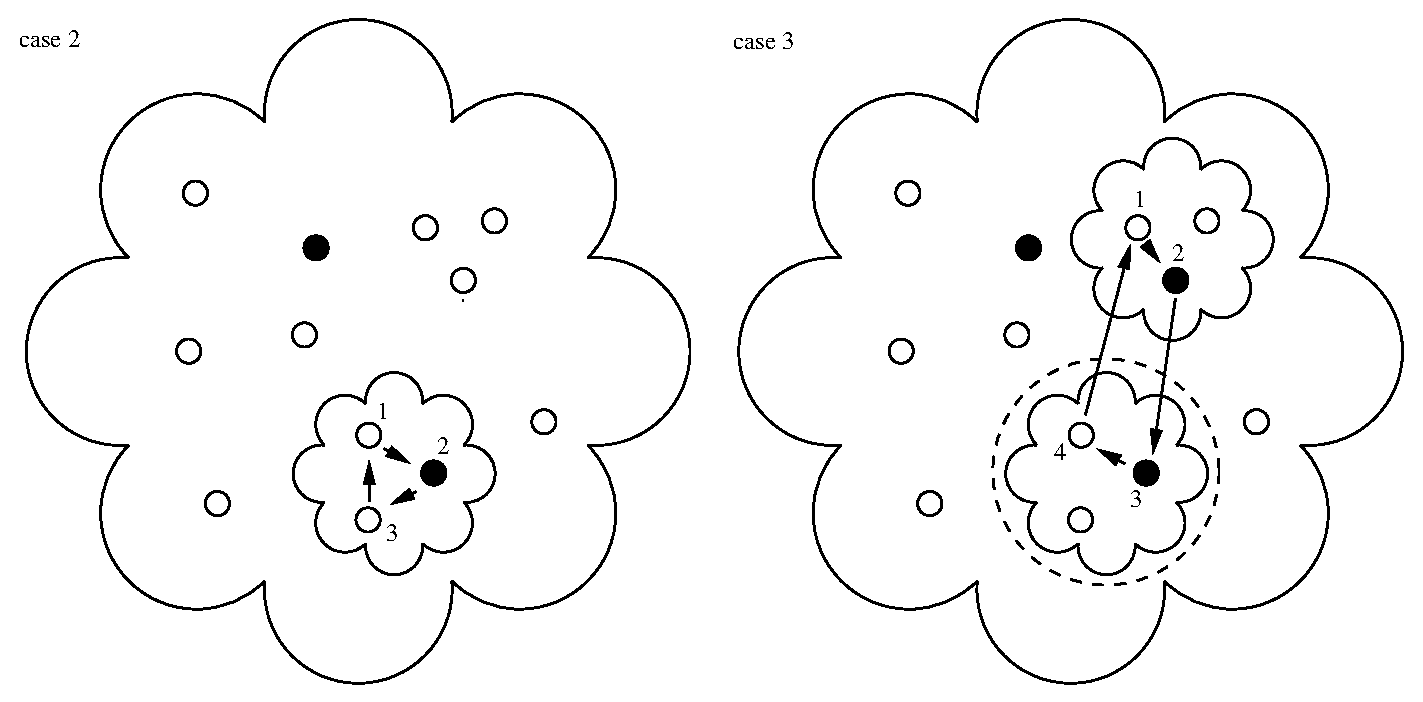
\includegraphics[scale=0.35]{FIGURES/ComGroup.eps} 
	\end{center}
          \caption{On the left: communications inside the same group. On the right: communications between two MPI-groups. The dashed circle indicates the group holding the requested data.
          In both cases, the master processes have a key role in distributing information for the exchange. Each arrow marks a request, the sequence of requests is enumerated.}  \label{MPIEXCHANGE}
\end{figure}

Clearly, smooth execution of any communication pattern arising from the great number of possible data dependencies
is key to a good performance of the Ambient approach. The resolution of communication patters also falls under the purview
of the packet manager, as it manages both intra- and inter-group communication. Each MPI-group has its own singleton packet manager.

To reach the best performance in HPC, bottlenecks arising from synchronization operations should be avoided  \cite{EXASCALE-2010}.
Thus, MPI asynchronous communication is privileged in Ambient (\texttt{mpi\_isend} and \texttt{mpi\_irecv}). As we avoid synchronization 
instructions, the process repeatedly checks for the availability of the incoming data in an infinite loop, until actually receiving the
data.

For the packet manager to be adaptable to any communication pattern, it employs the delegate mechanism and a finite state machine (FSM).

\begin{table}[b] 
	\begin{center}
	 	\begin{tabular}{l l }
                           \hline 
                           Algorithm of the packet manager   &    \\ \hline
                           \textbf{Require}  a MPI process requires a block of data &  \\                           
                            \begin{tabular}{c l}                                
                               \tiny{1:}   & \textbf{for}  ;;  \textbf{do} $\vartriangleright$  infinite loop \\
                               \tiny{2:}   & \hspace{0.2 cm}  \texttt{Delegate()}  $\vartriangleright$ check if packet has been \\
                                                & received, and re-send if needed \\
                               \tiny{3:}   & \hspace{0.2 cm}  FSM $\vartriangleright$ break the loop, \\
                                               & if all packets have arrived at destination. \\
                               \tiny{4:}   & \textbf{end do} \\
                           \end{tabular}   &  \\ \hline
        	     \end{tabular}
	\end{center}
	\caption{Description of the packet manager}
\end{table} 



%\begin{figure}[h]
%	\begin{center}
%	    \psfrag{1}{\tiny \hspace{-0.1 cm}  1}
%	    \psfrag{2}{\tiny \hspace{-0.1 cm}  2}
%	    \psfrag{Loose}{\tiny \hspace{-0.2 cm}   Loose}
%	    \psfrag{Closure}{\tiny \hspace{-0.2 cm}  Closure}
%	    \psfrag{Open}{\tiny \hspace{-0.4 cm}  Opening}
%          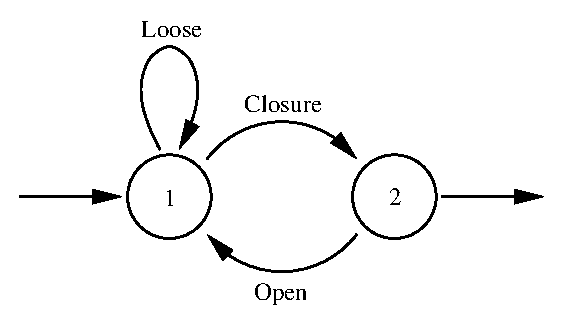
\includegraphics[scale=0.45]{FIGURES/FSM.eps} 
%	\end{center}
%          \caption{Schematic of the finite sate machine for the closing procedure. The states 1 and 2 correspond to open or close.
%           The transitions are loose, closure or opening, they  depend of the situation of all packets (if they all reach theirs targets or not),
%                          the loose transition means the packet has not been received, thus we iterate one more time on the infinite loop.}  \label{FSM}
%\end{figure}

The delegate mechanism serves its design goal - to execute handlers of components listening for the packets arrival, such as layout tables.
This delegate object inside the packet manager is tied to a list of functions, such as layout forwarding, 
data block forwarding and control information handlers. As the packet manager checks for completion of the local send process, the finite state machine
checks the send completion state of the other MPI processes (whether they have sent all their packets or not). If all the packets have been sent, the FSM breaks the infinite loop.


%%%%%%%%%%%%%%%%%%%%%%%%%%%%% END PACKET MANAGER 

%%%%%%%%%%%%%%%%%%%%%%%%%%%%% BEGIN ABSTRACT PARALLEL DATATYPES 
\subsection{Abstract parallel datatypes} \label{ABSTRACTPARADATATYPE}

In order to turn Ambient into a general purpose framework, we have decoupled the Ambient data representation from the user datatypes. There are two aspects to the parallel datatypes:

First is the object's lifetime. Due to the accumulated execution model, objects may be used after their lexical scope has expired.
For this purpose we introduced \texttt { livelong } class that forces derived data types to duplicate themselves in heap memory upon construction if they were allocated on stack. Using this duplicate we can ensure that the object will stay alive until the moment of execution of the actual kernels using this data. 

The second aspect is the actual connection to Ambient's work groups engine. Each data type derived from the livelong class has a field pointing to an associated parallel profile of the object. This parallel profile object is responsible for the data storage and actual tracking of the physical location of the data pieces throughout the cluster's processes. The relationship between user type and parallel profile is regulated by means of providing a specialized constructor for the user's data type that sets the memory storage parameters according to the actual user's object parameters in a user defined way. 

That is, one is free to design his own data types like e.g. a parallel sparse matrix type, either alongside the embedded parallel dense matrix type, or to replace it if the user chooses to. The simpliest example would be for a dense matrix. Inside the specialized constructor we simply set the \texttt{dim.x} and \texttt{dim.y} of the parallel profile to be the numbers of columns and rows respectively. Assuming the size of the work group is provided, this immidiately sets the work group grid of the object. Alongside with the dimension other parameters are being set - such as the data element size and the work block/work item dimensions (the latter can be changed individually for the object during runtime).

In general, the mechanism described above provides us with all means to adapt the framework in a simple and flexible way to any abstract parallel types that the user might want to use for computations.

%%%%%%%%%%%%%%%%%%%%%%%%%%%%% END ABSTRACT PARALLEL DATATYPES 


%%%%%%%%%%%%%%%%%%%%%%%%%%%%% BEGIN VALIDATION
\subsection{Validation}
As a validation test, we've coded a new implementation of PDGEMM using the Ambient framework, and compare to the ScaLAPACK version of PDGEMM (MKL-Version).
The algorithm of our implementation is based on the classical blocking method [CITATION NEEDED] using a column order distribution for the matrices (\cf table \ref{AMBIENTDGEMM} 
for the modification due to Ambient). One of the obvious advantages in our implementation is the required amount of coding, which is limited to seven lines in this case.

We compare the Ambient results with the ScaLAPACK implementation. As related in section \ref{CUDAIDEOLOGYSECTION}, Ambient is compatible with ScaLAPACK,
despite the difference in memory layout. In Ambient, each work group is principally independent from any other, even if they belong to the same process, while in ScaLAPACK
blocks are grouped by process s.t. a memory-contiguous object is obtained. Therefore, calling a ScaLAPACK solver from Ambient must entail rearrangement of appropriate
work groups into a contiguous blocks, and thus a certain overhead. Due to Ambients flexibility in handling and grouping data, from a programming perspective this task
is simple to accomplish however. 

 \begin{table}[t] 
	\begin{center}
	 	\begin{tabular}{l l }
                           \hline 
                           \textbf{ Algorithm:}  pDGEMM using Ambient  &    \\ \hline
                           \textbf{Require}                 A pinned computational kernel  &  \\
                           \begin{tabular}{c l} 
                                 \tiny{1:} &  Get the cartesian coordinate $i,j$ of the work group \\ 
                                 \tiny{2:} &  Refer  the  work group$(i,j)$  of B into $B_{ref}$ \\
                                 \tiny{3:} &  \textbf{for} from $k(0)$  to the max number of rows \textbf{do} \\
                                 \tiny{4:} &  \hspace{0.2 cm} Refer  the  work group$(k,j)$  of A into $A_{ref}$ \\    
                                 \tiny{5:} &  \hspace{0.2 cm}  reduction of the blocks $(k,i)$ into $C_{ref}$ , $\vartriangleright$  The reduction, \\
                                                & \hspace{0.2 cm}  is done by a proxy pattern \\
                                 \tiny{6:} &  \hspace{0.2 cm}  classical DGEMM($A_{ref}$, $B_{ref}$, $C_{ref}$)\\
                                 \tiny{7:} &  \textbf{end do} \\    
                             \end{tabular} & \\ \hline
		 \end{tabular} 
		 \caption{Algorithm of the pDGEMM using Ambient framework. We remember a proxy pattern is an interface the something else (object in memory). There, it allows the reduction between the independent workgroups.   \label{AMBIENTDGEMM}}
	\end{center}
\end{table} 

The validation test consists of multiplying matrices and saving the results into an output matrix, $C = A \times B$,
where we further compare between the output of the Ambient computational kernel and the ScaLAPACK PDGEMM solver.
Using the C++ language, the operations $\times$ and $=$ have been overloaded appropriately, now containing the "pushing" of the required logistic and computational kernels.
Afterwards, results are compared element by element using the test  \cite{Dongarra:1990:SLB:77626.79170}  $\left \lvert C^S_{ij} - C^A_{ij} \right \rvert/\left \lvert  \epsilon C^S_{ij} \right \rvert  < n$,
where  the precision factor $\epsilon$  is the \texttt{double} precision $10^{-16}$, indices  $S$ and $A$ represent the ScaLAPACK and the Ambient version, and $n=16$, the exponent of numerical precision. 

For the test, the size of work groups has been fixed to $128 \times 128$, and the square matrices $A$, $B$ range from 256 up to 8196 in size (step size of 128). The numbers of MPI-Process varied from 2 to 8.
Matrices were filled upusing a pseudo random number generator  \texttt{drand48()}\footnote{This function returns 
pseudo-random numbers non-negative, double-precision,  uniformly distributed over the interval $[0, 1]$ using a linear congruential algorithm and 
48-bit integer arithmetic. }  from \texttt{stdlib}.  
%%%%%%%%%%%%%%%%%%%%%%%%%%%%% END VALIDATION



%%%%%%%%%%%%%%%%%%%%%%%%%%%%% END DESCRIPTION OF THE FRAMEWORK

\section{Results and discussions}
\subsection{First benchmark case}
The first benchmark consists of evaluating the performance of our parallel matrix multiplication relative to the ScaLAPACK-MKL implementation. Both solvers are included as computational kernels
in Ambient.  The initial condition are the same than the validation test. As the validation test, the matrices size vary from 256 up to 8196 by step of (128 elements). A 1-D cyclic  column distribution is
used for both algorithm. As both kernels are included inside the framework additional workload should take into account and for the ScaLAPACK pDGEMM, we reorganize data to fit the ScaLAPACK
representation. The benchmarks  were performed on AMD Opteron  Magny-Cours) CPUs at 2.2 GHz on the Swiss National Supercomputing Centre facilities. The peak performance $P_m$ is reported in [GFlops], it is simply
calculated by :

\begin{eqnarray}
P_m  = \frac{2n^i}{t},
\end{eqnarray}
where $n$ is the size of the square-matrix,  $t$ the full time of calculation and $i$ is equal to 3 for the classical matrix multiplication algorithm.

\begin{figure}
\include{PLOT/SinglePDGEMM/SinglePGEMMWK}
\caption{Performances of PDGEMM using Ambient  \label{PLOTSINGLE0}}
\end{figure}

\begin{figure}
\include{PLOT/SinglePDGEMM/SinglePGEMMWKSCALA}
\caption{Comparing Ambient's PDGEMM against ScaLAPACK  \label{PLOTSINGLEq}}
\end{figure}

The benchmark of our Ambient pDGEMM is presented on the figure \ref{PLOTSINGLE0}


\subsection{Second benchmark case}
This benchmarks  evaluates the global performance of the scheduler, especially, when  the independent operations are executed all over the cluster. 
We now multiply two vectors of matrices pair by pair. Every multiplication is performed by 2 MPI process and the size of the vectors vary from to
1 to 48. Thus, the final number of MPI process is equal to 96 which corresponds to fill up 4 calculation nodes.

Before presenting and commenting the results, we would like highlight the readers of the programming of this benchmark. The coding simply consists of few lines
of declarations, initializations and a basic loop for, as we presented into the algorithm \ref{EXECUTION}. Naturally, coded algorithm  integrates two levels of distributed parallelization 
without integrate any MPI instructions.
 
In this benchmark, we  plot the ratio between the performance peak of  vector of matrices $P_{v_m}$ and the associated peak of the machine $P_m$. It is expressed by 
$R = P_{v_m}/P_m$, or developed by :

\begin{eqnarray}
R = 100\frac{2n^3 N_m }{4f t N_p},
\end{eqnarray}
where $N_m$ is the number of matrices, $N_p$ the number of processor, $t$ the full time of execution and $f$ the frequency of the processor. Results are presented on the figure \ref{PLOTVECTOR0}
 

\begin{figure}
\include{PLOT/VectorPDGEMM/VectorWL0}
\caption{Peak performance ration of a variable vector of matrices. \label{PLOTVECTOR0}}
\end{figure}

\begin{figure}
\include{PLOT/VectorPDGEMM/VectorWL_2}	
\caption{something else}
\end{figure}

 	
\subsection{Third benchmark case}





\section{Conclusions}

%%%%%%%%%%%%%%%%%%%%%%%%%%%%% BEGIN THANK 
\thanks{The authors are grateful to W. Sawyer and G. Fourestey from the CSCS staff and V. Rezzonico from EPFL.} 
%%%%%%%%%%%%%%%%%%%%%%%%%%%%% END THANK 



%%%%%%%%%%%%%%%%%%%%%%%%%%%%% BEGIN BIBLIO
\bibliographystyle{abbrv}
\bibliography{biblio}
%%%%%%%%%%%%%%%%%%%%%%%%%%%%% END BIBLIOr



\end{document}  
